\documentclass[a4paper]{article}

\usepackage[T1]{fontenc}
\usepackage[utf8]{inputenc}
\usepackage[swedish]{babel}
\usepackage{fancyhdr}	
\usepackage{graphicx}

\lhead{Felix Hedenström \\ Jonathan Rinnarv}
\chead{19940922-1737 \\19930121-3634}
\rhead{fhede@kth.se \\rinnarv@kth.se}
\pagestyle{fancy}

\begin{document}
\title{Labbrapport Logik - Modellprovning för CTL}
\author{DD1350 Logik för dataloger \\ Felix Hedenström\\ Jonathan Rinnarv}
\maketitle
\thispagestyle{empty}
\newpage
\tableofcontents
\thispagestyle{empty}
\newpage
\setcounter{page}{1}.
\section{Inledning}
Genom denna laboration implementerade vi ett program för att undersöka om en viss modell är valid. Vi gjorde detta genom språket Prolog då det är bra på rekursiva förgreningsanrop, vilket är viktigt i CTL modeller.  

Programmet undersöktes genom att testa 1213 modeller. Av dessa var 483 tänkt att resultera i ett svar att de var icke fungerande modeller, och 730 skulle resultera i att modellerna stämde. Iterativt förbättrades programmet tills det fick förväntade resultat på alla testerna.

\subsection{Frågeställning}
\begin{itemize}
\item Hur hanterar man regler som kräver ett ospecificerat antal indata?
\item Vilka hjälp-predikat kommer vara viktiga?
\item Kan vi skapa en intressant modell? Kan vi visa exempel på formler som håller och inte håller i denna modell?
\end{itemize}
\section{Metod}
Först implementerades enkla, egenskapade versioner av alla regler. Dessa testades mot de testfallen som skulle hålla. Först användes egenskapade testfall med mycket enkla modeller, för att testa reglerna en och en. Sedan testades kombinationer av regler och mer avancerade modeller skapades.

Efter de enklare testfallen var avklarade gick det vidare till det stora biblioteket av testfall. Testfallen gicks igenom en och en till felaktigt resultat hittades. För snabbare komma fram till ett bra program användes CTL-reglerna för att förbättra de regler som redan hade implementerats, istället för att komma på egna helt sunda regler. 

Eventuella felaktiga resultat debuggades. Ofta löste sig flera felaktiga resultat i taget, vilket visade på att många testfall delar egenskaper.
\section{Resultat}
\subsection{Algoritmbeskrivning}
Mycket av programmet var enkelt implementerat på grund av Prologs paradigm. Prolog söker enkelt igenom alla möjliga tillstånd genom djupet-först rekursion när det behövs. Alla regler börjar appliceras från första tillståndet och tar sig sedan därifrån om regeln kräver det. Ofta är det regler med flera djup, vilket kräver att man undersöker flera nivåer av egenskaper. 

Ett hjälppredikat som avgjorde grannarna till ett visst tillstånd. Samma hjälpmetod kunde även användas för att avgöra egenskaperna för en visst tillstånd. Denna metod byggde mycket på idén av en hashmap. Den tog in en ''hashmap'', en ''key'', och tog fram ett ''value''. 
\subsection{Ospecificerat antal indata}
För regler som kräver ospecifierat antal data, såsom AG, användes predikatet \emph{forall}. Det användes ofta som:\\
\begin{verbatim}
forall(members(X,Grannar),check(T,L,X,[S|U],ag(F))
\end{verbatim}
Det går då igenom alla \emph{X} som finns i listan och är sant om check(...) är sant för alla olika X.
\subsection{Predikat}
\begin{tabular}{|p{3.1cm}|p{2.75cm}|p{2.75cm}|p{2.75cm}|}
\hline
\textbf{Predikat} & \textbf{Sant} & \textbf{Falskt} & \textbf{Kommentar}\\
\hline
verify($+$Input) & När input följer är en valid modell. & När input inte är en valid modell. & Används för att dela upp grannlista, egenskapslista, starttillstånd och en CTL-formel.\\
\hline
check($+$Grannlista, $+$Egenskapslista, $+$Tillstånd, $+$Besökta\_tillstånd, $+$CTL-formel) & När CTL-formeln gäller för i det Tillstånds som är. & När CTL-formeln inte gäller. & Om regeln har djup går predikatet igenom alla nivåer av predikatet.\\
\hline
getValue($+$List, $+$Key, $?$Value) & Om Value är det värdet som Key:n pekar på.  & När Key:n inte finns i List. & Om List är grannlistan och Key är ett tillstånd kommer Value vara alla grannar till Key:n.\\
\hline
\end{tabular}
\newpage
\section{Appendix A - Mastermind Modell}
\begin{figure}
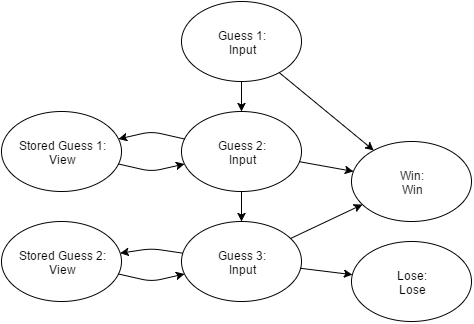
\includegraphics[width = \textwidth]{modell.jpg}
\caption{Modell över förenkelat mastermind - Starttillstånd Guess 1}
\end{figure}

\subsection{Valid CTL formel}
$$AG (EF ((Win \lor Lose)))$$
Oavsätt vilket tillstånd du är i kan du ta dig till Win eller Lose. Detta är självklart för de flesta enkla spel där man kan antingen vinna eller förlora.
\subsection{Icke-valid CTL formel}
$$AG (View \lor EX(Win))$$
Antingen är man på ett tillstånd med View-egenskapen, eller så kan man ta sig till Win nästa drag. Detta betyder att man antingen kollar på sina tidigare gissningar, eller så kan man vinna inom nästa drag. Detta stämmer faktiskt för alla tillstånd i modellen, förutom ett, när man är i Lose tillståndet. Då är man inte på view tillståndet och man kan icke ta sig till Win. 
\section{Appendix B - Kod}
\begin{verbatim}
% For SICStus, uncomment line below: (needed for member/2)
%:- use_module(library(lists)).
% Load model, initial state and formula from file.
verify(Input) :-
	see(Input), read(T), read(L), read(S), read(F), seen,
	check(T, L, S, [], F),
	!.
% check(T, L, S, U, F)
%     T - The transitions in form of adjacency lists
%     L - The labeling
%     S - Current state
%     U - Currently recorded states
%     F - CTL Formula to check.
%
% Should evaluate to true iff the sequent below is valid.
%
% (T,L), S  |-    F
%             U
% To execute: consult('your_file.pl'). verify('input.txt').

getValue([[Key|[Return_list]]|_],Key,Return_list):- !.

getValue([_|T],Key,Return_list):-
	getValue(T,Key,Return_list).


% Checks if F and G are true at S
check(T,L,S,_, and(F,G)):-
	check(T,L,S,[],F),
	check(T,L,S,[],G).


% Checks if F or G is true at S
check(T, L, S, _, or(F,G)):-
	check(T,L,S,[],F); 
	check(T,L,S,[],G).


% I alla nästa tillstånd ska F gälla. Man tittar
% alltså inte nödvändigtvis på sig själv om man 
% inte har en loop som går tillbaka till sig själv
check(T,L,S,_,ax(F)):-
	getValue(T,S,S_NEXTS),
	forall(member(X,S_NEXTS),check(T,L,X,[],F)).

% I något nästa tillstånd ska F gälla. 
% Man behöver inte titta på sig själv
check(T,L,S,_,ex(F)):-
	getValue(T,S,S_NEXTS),
	member(X,S_NEXTS),
	check(T,L,X,[],F).


% AG1
check(T, L, S, U, ag(F)):-
	member(S,U),
	check(T, L, S, [], F).

% AG2
check(T , L, S, U, ag(F)):-
	not(member(S,U)),
	check(T, L, S, [], F),
	getValue(T,S,S_NEXTS),	
	forall(member(X,S_NEXTS), check(T,L,X,[S|U],ag(F))).

% EG1
check(_,_,S, U, eg(_)):-
	member(S,U).

% EG2
check(T , L, S, U, eg(F)):-
	not(member(S,U)),
	check(T, L, S, [], F),
	getValue(T,S,S_NEXTS),
	member(X, S_NEXTS),
	check(T, L, X, [S|U], eg(F)).

% AF1
check(T , L, S, U, af(F)):-
	not(member(S,U)),
	check(T,L,S,[],F).

% AF2
check(T, L, S, U, af(F)):-
	not(member(S,U)),
	getValue(T,S,S_NEXTS),
	forall(member(X,S_NEXTS), check(T,L,X,[S|U],af(F))).

% EF1
check(T, L, S, U, ef(F)):-
	not(member(S,U)),
	check(T,L,S,[],F).

% EF2
check(T,L,S,U,ef(F)):-
	not(member(S,U)),
	getValue(T,S,S_NEXTS),
	member(X,S_NEXTS),
	check(T,L,X,[S|U],ef(F)).

% If X is not present at L(s) this predicate is true
check(_, L, S, [], neg(X)) :- 
	getValue(L,S,List),
	not(member(X,List)).

% If X is present at L(s)
check(_ , L, S, [], X):-
	getValue(L,S,List),
	member(X,List).
\end{verbatim}
\end{document}
